			\documentclass{article}
			\usepackage[margin=1.25in]{geometry}
			\usepackage{graphicx}
			\usepackage{listings}
			\usepackage{titlepic}
			\usepackage{afterpage}
\usepackage{textcomp}
			\usepackage{float}
\usepackage[figuresleft]{rotating}
			\usepackage{hyperref}
\usepackage{xcolor}
			\newcommand\tab[1][1cm]{\hspace*{#1}}
			\usepackage{multicol}
			\renewcommand{\labelenumii}{\theenumii}
			\newcommand{\quotes}[1]{``#1''}
			\renewcommand{\theenumii}{\theenumi.\arabic{enumii}.}
			
			\begin{document}
			\title{
\includegraphics[scale = .6]{uom.png}
				\linebreak 
				\textbf{CPS2000 - Compiler Theory \& Practise}\linebreak\linebreak
				\textbf{Assignment Part 2}\linebreak\linebreak
				\large{B.Sc Computer Science}
				\date{}
				\author{Jacques Vella Critien - 97500L}}
				
				\begin{titlepage}
					\maketitle
					\thispagestyle{empty}
				\end{titlepage}
				
				\tableofcontents
				\newpage
				
				\section{Task1: Extending SmallLang}
				
				For the first task of this part of the assignment, we were required to extend SmallLang into SmallLangV2 by adding some other features. These features include adding support for the primitive type \quotes{char} and for arrays which hold a series of elements of the same type in contiguous memory. It was required to let array values uninitialised by default but an implementation for initialisation for values was also required. Moreover, formal parameters had to be changed in order to support both the \quotes{char} type and the arrays as types. In order to implement this, as can be seen below, EBNF rules had to be added and some were changed.
				
				\subsection{Solution}
				
				The rules below show the new and changed rules. The other rules which were present in SmallLang and not included in the below set, have not changed.
				
				\begin{lstlisting}[backgroundcolor=\color{lightgray},basicstyle=\small,upquote=true]
				
  <ArraySizeIndex> 	::= '[' <Expression> ']'
  
  <ArrayIdentifier> 	::= <Identifier> <ArraySizeIndex>
  
  <ArrayValue> 		::= '{' <Expression> { ',' <Expression> } '}'
  
  <VariableDecl> ::= <Identifier> ':' (<Type>|<Auto>) '=' <Expression> 
  
  <ArrayDecl> 	::=  <ArrayIdentifier>`:' <Type> ['=' <ArrayValue>] 
  
  <FormalParam> 	::= <Identifier> [ '[' ']' ] : <Type>
  
  <AbstractIdentifier>	::= <Identifier> | <ArrayIdentifier>
  
  <Assignment>	::= <AbstractIdentifier> `=' <Expression>
  
  <Decl> 		::= 'let' (<VariableDecl> | <ArrayDecl>)
  
  <CharLiteral>  	::= '\'' <Letter> '\''
  
  <Literal> 		::= <BooleanLiteral>
  			 |  <IntegerLiteral>
  			 |  <FloatLiteral>
  			 |  <CharLiteral>
  					
  <Factor> 		::= <Literal>
  			 |  <AbstractIdentifier>
  			 |  <FunctionCall>
  			 |  <SubExpression>
  			 |  <Unary>
  
  <Statement> 		::= <Decl> ';'
  			|   <Assignment ';'
  			|   <PrintStatement> ';'
  			|   <IfStatement> 
  			|   <ForStatement> 
  			|   <WhileStatement> 
  			|   <RtrnStatement> ';'
  			|   <FunctionDecl>
  			|   <Block>
  
  
  	
				  
				\end{lstlisting}
				
				
				\subsubsection{\textless ArraySizeIndex\textgreater}
				
				This rule represents the size of the array in the case of a declaration while it represents the index to assign in an assignment. It consists of an expression in the middle of square brackets.
				
				\subsubsection{\textless ArrayIdentifier\textgreater}
				
				This rule represents an array identifier and it consists of an identifier followed by the above rule, which represents the size or the index.
				
				\subsubsection{\textless ArrayValue\textgreater}
				
				This rule represents the value to set to the array on declaration. This consists of an expression or more inside curly brackets.
				
				\subsubsection{\textless VariableDecl\textgreater}
				
				This rule represents a variable declaration for an array. I updated it by removing the 'let' from the start and starting with an <Identifier> node before a semi colon and a type which can also be auto. Finally, it remains the same by expecting an equal sign and an expression
				
				\subsubsection{\textless ArrayDecl\textgreater}
				
				This rule represents the declaration for an array. It starts with an \textless ArrayIdentifier\textgreater{} node explained above before a semi colon and a type. As can be seen in the figure above, an equals sign and an \textless ArrayValue\textgreater{} node are optional because arrays can be initialised or uninitailised in declarations.
				
				
				\subsubsection{\textless Decl\textgreater}
				
				Similarly, this new rule just represents either a variable declaration or an array declaration node by first expecting a let and then, either type of declaration.
				
								\subsubsection{\textless Assignment\textgreater}
				
								This rule is an updated version of the \textless Assignment\textgreater{} rule from part 1 of this assignment. As can be seen, this rule now accepts an ASTAbstractIdentifier which includes both ASTArrayIdentifier and ASTIdentifier rather than just ASTIdentifier.
				
				
				\subsubsection{\textless FormalParam\textgreater}
				
				This rule is an updated version of the \textless FormalParam\textgreater{} rule from part 1 of this assignment. As can be seen, optional empty square brackets are possible after the identifier which indicates an array as a formal parameter. Despite it is listed as an identifier, the actual code in the parser looks for a trailing `[` and if it is found an ASTArrayIdentifier node is returned and not an ASTIdentifier.
				
				\subsubsection{\textless AbstractIdentifier\textgreater}
				
				This new rule just represents either a normal identifier or an array identifier rule.
								
				
				\subsubsection{\textless CharLiteral\textgreater}
				
				This new rule was added to represent a character literal and it consists of a \textless Letter\textgreater{} rule in between two apostrophes.
				
				\subsubsection{\textless Literal\textgreater}
				
				This rule represents a literal and was updated to be able to also represent a \textless CharLiteral\textgreater {} rule.
				
				\subsubsection{\textless Factor\textgreater}
				
				This rule was updated to be able to represent an \textless AbstractIdentifier\textgreater{} rule instead of an \textless Identifier\textgreater{} rule to be able to also represent an \textless ArrayIdentifier\textgreater{} rule.
				
				\subsubsection{\textless Statement\textgreater}
				
				This rule was updated to be able to represent a \textless Decl\textgreater{} rule instead of an \textless VariableDecl\textgreater{} rule to be able to also represent an \textless ArrayDecl\textgreater{} rule.
				
				
				\section{Task1: SmallLangV2 Lexer and Parser}
				
				The second task required was to implement the necessary changes for the lexer and parser in order to process the input program containing the new features, namely the character literal and arrays. In order to perform this, I started off by extending the DFA (Deterministic Finite Automaton) to be able to split the inputs into correct tokens. Moreover, as will be explained below, the three tables which are the \quotes{Classifier Table}, the \quotes{Type Token Table} and the \quotes{Transition table} were also changed. Finally, for the parser, new nodes were created and the Parser class was updated. 
				
				\subsection{Deterministic Finite Automaton}
				
				The figure below shows the added items to the automaton in part 1 so that the new features can be applied. As can be easily seen, State S28 represents a `[' token, State S29 represents the `]' token and S32 represents a character literal token, whose lexeme is in the form of `\textless character\textgreater'. \textbf{Once again, it is important to note that for each state, any other character inserted which are not visible in the paths going out from that state ALL lead to an absorbing bad state. This is not included in the diagram just to keep the diagram clear.}
				
				\begin{center}
					\begin{figure}[H]
			 			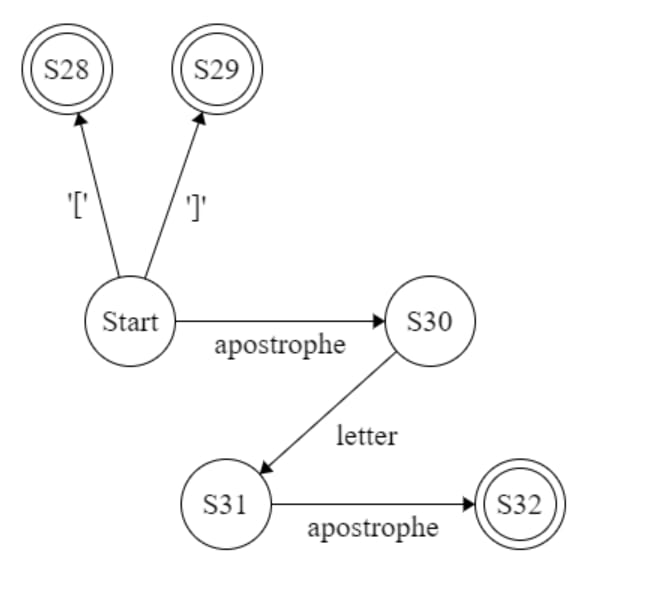
\includegraphics[width=0.6\textwidth]{part2automaton.jpeg}
			 			\centering
			  			\caption{Deterministic finite automaton additions}
			  			\label{fig:automaton}
					\end{figure}
				\end{center}
				

			\subsection{Tables}
			\subsubsection{Classifier Table}
			
			This table which relates the specific characters of input to the classifiers was updated in order to support the three new classifiers or categories. The new classifiers can be seen below and these were added to the the Classifier table created for part 1 of the assignment. The top row shows the character inputted and the bottom row shows the related classifier.
			
			 \begin{center}
					\begin{figure}[H]
			 			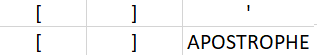
\includegraphics[width=0.4\textwidth]{ctpart2.png}
			 			\centering
			  			\caption{Classifier Table additions}
			  			\label{fig:cttable}
					\end{figure}
				\end{center}
				
				\subsubsection{Type Token Table}
			
			This table which relates states to the classifiers was updated in order to support the five new states. The new states can be seen below and these were added to the the Type Token table created for part 1 of the assignment. The top row shows the state and the bottom row shows the related classifier.
			
			 \begin{center}
					\begin{figure}[H]
			 			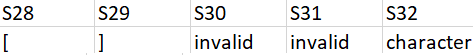
\includegraphics[width=0.6\textwidth]{ttpart2.png}
			 			\centering
			  			\caption{Type Token Table additions}
			  			\label{fig:tttable}
					\end{figure}
				\end{center}
				
				
				\subsubsection{Transition Table}
			
			This table which represents transitions from one state to another state when given a classifier, was updated in order to add the three new classifiers and the five new states. The transitions involving the new classifiers and states can be seen below marked in red. This was done to be able to distinguish them from previously created transitions for part 1 of the assignment. The columns represent the classifiers while the rows represent the states.
			
			 \begin{sidewaysfigure}
			 			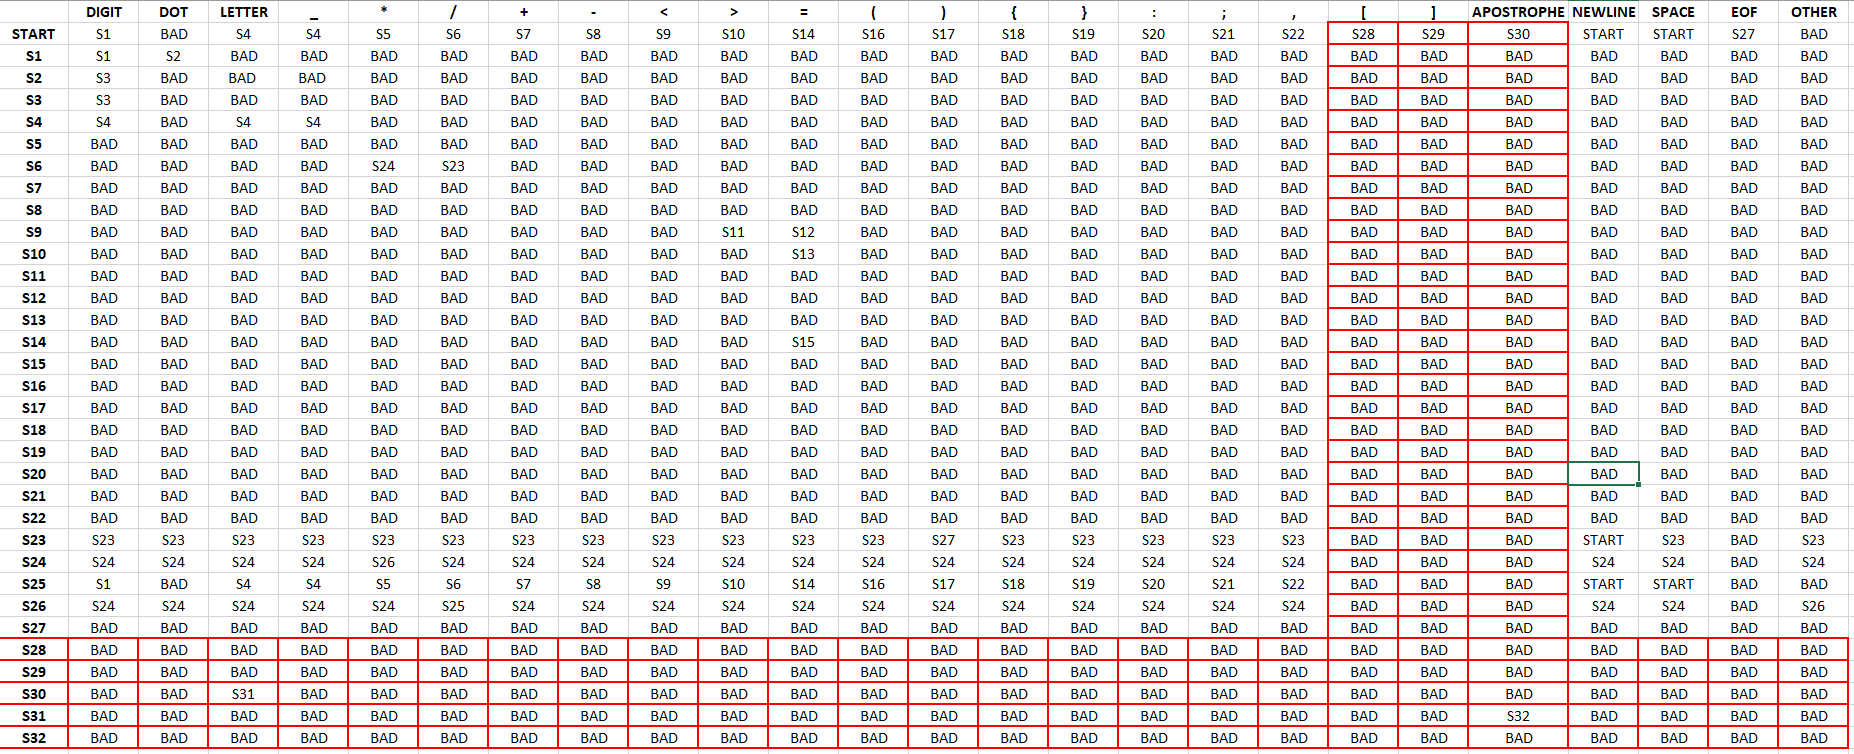
\includegraphics[width=\textwidth]{txpart2.png}
			 			\centering
			  			\caption{Transition Table additions}
			  			\label{fig:txtable}
				\end{sidewaysfigure}
			
			\pagebreak
			
			\subsection{Lexer Solution}
			
			This section highlights and explains the difference and additions made in the code to support these new features in relation to the \textbf{lexer}.
			
			\subsubsection{TypeToken.java}
					
					This enum class which holds the different types of tokens was updated to include the following:
					\begin{itemize}
						\item SQUARE\_OPEN
						\item SQUARE\_CLOSE
						\item CHARACTER\_LITERAL
					\end{itemize}
				
				\subsubsection{Category.java}
					
					This enum class which holds the different types of categories or classifiers was updated to include these three new classifiers:
					\begin{itemize}
						\item SQUARE\_OPEN
						\item SQUARE\_CLOSE
    						\item APOSTROPHE
					\end{itemize}
					
				      \subsubsection{State.java}
					
					This enum class which holds the different types of states was updated to include these 5 new states:
					\begin{itemize}
						\item S28
						\item S29
    						\item S30
    						\item S31
    						\item S32
					\end{itemize}
					
					\subsubsection{Keyword.java}
					
					This class which extends the Token class and in which all the keywords in the SmallLangV2 syntax are declared was updated and a new keyword to represent the char primitive was created and defined with the name CHAR.
					
					\subsubsection{Lexer.java}
					
					This class which contains all the methods needed from the parser to obtain the next token was updated to be able to handle the new features. Below contains all the list of methods that were changed and how:
					
					\begin{enumerate}
					\item \textbf{setTransitionTable()}: This function which populates the transition table hashmap was updated by adding the new transitions involved with the new classifiers and states. Basically, all the added transitions are the ones marked in red in the figure found in section 2.2.3
					\item \textbf{setAcceptableStates()}: This function which populates the acceptable states hashmap was updated to include set states S28, S29 and S32 as acceptable states. These states can be confirmed as being acceptable and final from the automaton on section 2.1 and the Type Token table in section 2.2.2.
						\item \textbf{charCat()}: This function which returns the category of a particular character was updated to support the three new tokens and categories which can be found in the classifier table in section 2.2.1
						\item \textbf{nextToken()}: This method which is called by the parser to give out the next token was only changed in the last part, that is the result reporting by adding a clause to check if it is a character literal and if so, the apostrophes are removed from the lexeme. This can be seen from the code snippet below.
					\begin{center}
					\begin{figure}[H]
			 			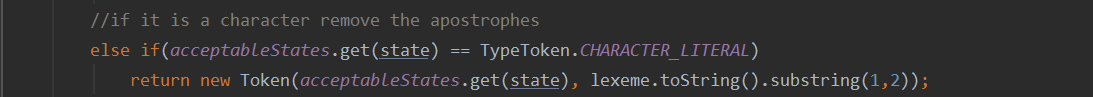
\includegraphics[width=0.8\textwidth]{lexerchange.png}
			 			\centering
			  			\caption{Change in nextToken() method}
			  			\label{fig:lexerchange}
					\end{figure}
				\end{center}
						
					\end{enumerate}
					

		\subsection{Parser Solution}
		
		This section highlights and explains the difference and additions made in the code to support these new features in relation to the \textbf{parser}.
		
		\subsubsection{ASTAbstractIdentifier.java}
					
					This is a class which extends the \textbf{ASTExpression} interface. This is extended by the \textbf{ASTIdentifier} and \textbf{ASTArrayIdentifier} classes. This class has the following 2 members: 
					\begin{enumerate}
					\item \textbf{name}: Its type is String and it is used to hold the variable name
					\item \textbf{type}: Its of type Type (enumeration) and it is used to hold the type of the identifier.
				
					\end{enumerate}
			In addition, this has getters for each member and a setter for the type to be used in case the identifier is of type auto so that it could be set to the expression's type as I will be explaining later.
			
			\begin{figure}[H]
					\centering
			 			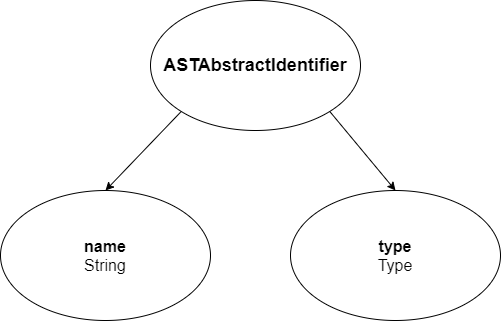
\includegraphics[width=0.55\textwidth]{astabstractid.png}
			  			\caption{ASTAbstractIdentifier node}
			  			\label{fig:astabstractid}
					\end{figure}
	
					
					
		\subsubsection{ASTIdentifier.java}
					
					This is a class which was created in part 1 of this assignment to represent an identifier. Now, it has been changed to extend the \textbf{ASTAbstractIdentifier} class and take up all of its member variables and methods which were explained in the above subsection highlighting the \textbf{ASTAbstractIdentifier} class.
					
					\begin{figure}[H]
					\centering
			 			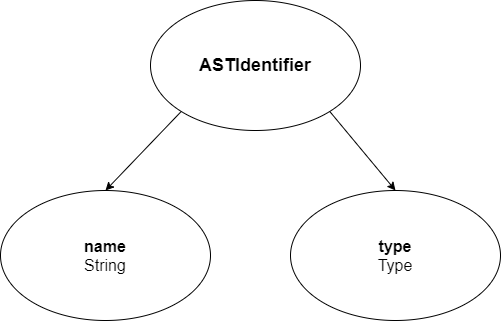
\includegraphics[width=0.55\textwidth]{astidentifier.png}
			  			\caption{ASTIdentifier node}
			  			\label{fig:astidentifier}
					\end{figure}
					
							\subsubsection{ASTArrayIdentifier.java}
					
					This is a class which extends the \textbf{ASTExpression} interface. This is extended by the \textbf{ASTIdentifier} and \textbf{ASTArrayIdentifier} classes. This class has the following 3 members: 
					\begin{enumerate}
					\item \textbf{name}: Its type is String and it is used to hold the variable name
					\item \textbf{sizeIndex}: Its of type ASTExpression and it is used to hold the size or index of the array identifier.
					\item \textbf{type}: Its of type Type (enumeration) and it is used to hold the type of the identifier.
				
					\end{enumerate}
			In addition, this has getters for each member, some of which are inherited from the ASTAbstractIdentifier class.
					
								\begin{figure}[H]
					\centering
			 			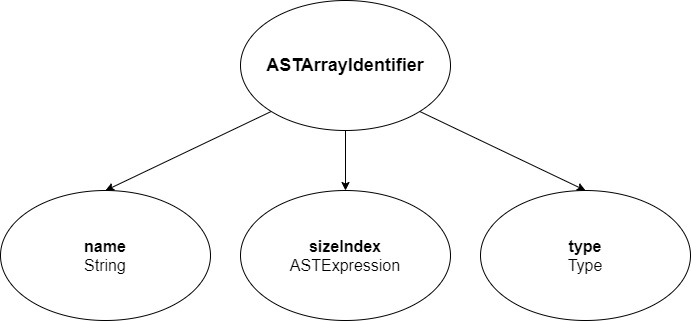
\includegraphics[width=0.55\textwidth]{astarrayidentifier.png}
			  			\caption{ASTArrayIdentifier node}
			  			\label{fig:astarrayidentifier}
					\end{figure}
					
							\subsubsection{ASTArrayValue.java}
					
					This is a class which extends the \textbf{ASTNode} interface. This was created to represent the value used to initialise an array, This class also has a member variable named values which is an arraylist of expressions of the type \textbf{ASTExpression}. In addition, this class also consists of constructors to create an object of this type,
					
								\begin{figure}[H]
					\centering
			 			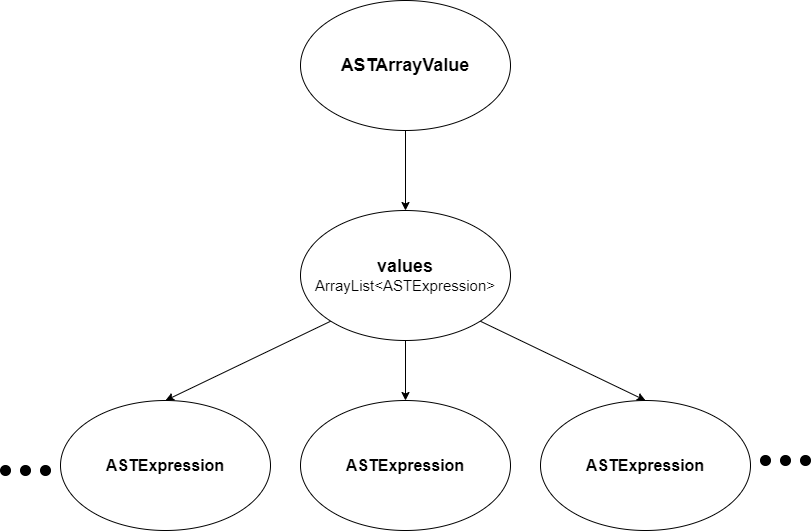
\includegraphics[width=0.55\textwidth]{astarrayvalue.png}
			  			\caption{ASTArrayValue node}
			  			\label{fig:astarrayvalue}
					\end{figure}					
					
										\subsubsection{ASTDecl.java}
					
					This is a class which extends the \textbf{ASTStatement} interface. This is extended by the \textbf{ASTVariableDecl} and \textbf{ASTArrayDecl} classes.
					
										\subsubsection{ASTVariableDecl.java}
					
					This is a class represents a variable declaration and was declared in part 1 of this assignment. The only change to this class was to make it extend the \textbf{ASTDecl} class.
					
					\subsubsection{ASTArrayDecl.java}
					
					This class was added to represent an array declaration. It extends the newly ASTDecl class and contains the following two member variables:
					
					\begin{enumerate}
					\item \textbf{values}: Its type is ASTArrayValue and it is used to hold the array values to be declared. This can be left empty if the array is declared but not initialised.
					\item \textbf{identifier}: Its of type ASTArrayIdentifier and it is used to identifier of the newly created array
				
					\end{enumerate}
			In addition, this also contains a constructor to create a new instance of this class.
			
							\begin{figure}[H]
					\centering
			 			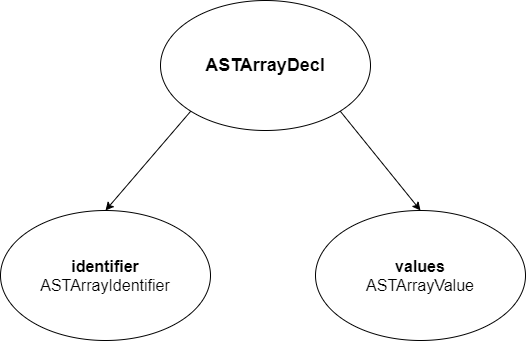
\includegraphics[width=0.4\textwidth]{arraydecl.png}
			  			\caption{ASTArrayDecl node}
			  			\label{fig:astarraydecl}
					\end{figure}
					
					
					\subsubsection{ASTAssignment.java}
					
					This is a class which was created in part 1 of this assignment to represent an assignment. Now, it has been changed so that its member variable which represents the \textbf{identifier} is changed to be of the type of ASTAbstractIdentifier instead of ASTIdentifier so that it would support both an ASTIdentifier and an ASTArrayIdentifier.
					
					\begin{figure}[H]
					\centering
			 			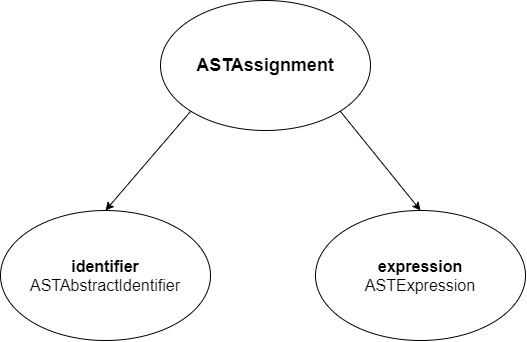
\includegraphics[width=0.55\textwidth]{astassignment2.png}
			  			\caption{ASTAssignment node}
			  			\label{fig:astassignment}
					\end{figure}
					
						\subsubsection{ASTFormalParam.java}
					
					This is a class which was created in part 1 of this assignment to represent a formal parameter. Now, it has been changed so that its member variable which represents the \textbf{identifier} is changed to be of the type of ASTAbstractIdentifier instead of ASTIdentifier so that it would support both an ASTIdentifier and an ASTArrayIdentifier
					
					\begin{figure}[H]
					\centering
			 			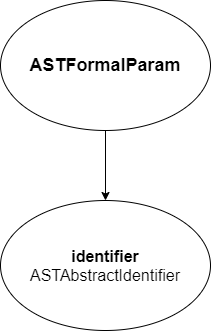
\includegraphics[width=0.25\textwidth]{astformalparam2.png}
			  			\caption{ASTFormalParam node}
			  			\label{fig:astformalparam}
					\end{figure}
					
				\subsubsection{ASTCharacterLiteral}
				
				This class was added to the other AST classes. This class extends the \textbf{ASTExpression} class and represents a char literal. This class contains only one member variable name \textbf{value} and a constructor.
				
				\begin{figure}[H]
					\centering
			 			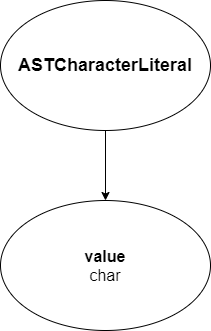
\includegraphics[width=0.25\textwidth]{ASTCharLiteral.png}
			  			\caption{ASTCharacterLiteral node}
			  			\label{fig:astcharlit}
					\end{figure}
				
				
				
				
				
				
				
				
		
		\bibliographystyle{ieeetr}
		\nocite{*}
\bibliography{references2}
			
		
			
					
			\end{document}